\documentclass[12pt,a4paper,]{article}
\newcommand*{\authorfont}{\fontfamily{phv}\selectfont}
\usepackage[]{libertine}
% If you're using libertine, this math font looks nice:
\usepackage[libertine]{newtxmath}
\usepackage[T1]{fontenc}
\usepackage[scaled=.95]{inconsolata}
% Add the following packages to support kableExtra
\usepackage{booktabs}
\usepackage{longtable}
\usepackage{array}
\usepackage{multirow}
\usepackage{wrapfig}
\usepackage{colortbl}
\usepackage{pdflscape}
\usepackage{tabu}
\usepackage{threeparttable}
\usepackage{threeparttablex}
\usepackage[normalem]{ulem}
\usepackage{makecell}
\usepackage{etoolbox}
% Uncomment the line below if you want to use XeLaTeX or 
% write on ShareLaTeX or Overleaf
% \setmonofont[Scale=.9,BoldFont=inconsolata-bold.ttf]{inconsolata-regular.ttf}
\usepackage[usenames,dvipsnames]{xcolor}
\definecolor{darkblue}{rgb}{0.0,0.0,0.55}
\usepackage{setspace}
\usepackage[top=2cm,bottom=2cm,left=2.2cm,right=2.2cm]{geometry}
\usepackage[backref,pagebackref]{hyperref}
\usepackage{dcolumn}
\usepackage{graphicx}
\usepackage{float}
\floatplacement{figure}{H}
\usepackage{pgf}
\usepackage{tikz}
\usetikzlibrary{arrows}
\usetikzlibrary{positioning}
\usepackage{mathtools}
\usepackage{caption}
\usepackage{ifthen}
\usepackage[UKenglish]{babel}
\usepackage[UKenglish]{isodate}
\cleanlookdateon
\exhyphenpenalty=1000
\hyphenpenalty=1000
\widowpenalty=1000
\clubpenalty=1000
\renewcommand*{\backref}[1]{}
\renewcommand*{\backrefalt}[4]{%
    \ifcase #1 (Not cited.)%
    \or        Cited on page~#2.%
    \else      Cited on pages~#2.%
    \fi}
\renewcommand{\backreftwosep}{ and~} 
\renewcommand{\backreflastsep}{ and~}
\hypersetup{
  linkcolor=Mahogany,
  citecolor=Mahogany,
  urlcolor=darkblue, 
  breaklinks=true, 
  colorlinks=true,
      pdfauthor={Danilo Freire; John Meadowcroft; David Skarbek; Eugenia Guerrero},
      pdfkeywords={Chile, georeferenced event data, human rights, Pinochet, truth
commission},
  }
\setlength{\parindent}{1cm}
\usepackage{ifxetex,ifluatex}
\usepackage{fixltx2e} % provides \textsubscript
\ifnum 0\ifxetex 1\fi\ifluatex 1\fi=0 % if pdftex
  \usepackage[T1]{fontenc}
  \usepackage[utf8]{inputenc}
\else % if luatex or xelatex
  \ifxetex
    \usepackage{amssymb,amsmath}
    \usepackage{mathspec}
  \else
    \usepackage{fontspec}
  \fi
  \defaultfontfeatures{Ligatures=TeX,Scale=MatchLowercase}
\fi
% use upquote if available, for straight quotes in verbatim environments
\IfFileExists{upquote.sty}{\usepackage{upquote}}{}
% use microtype if available
\IfFileExists{microtype.sty}{%
\usepackage{microtype}
\UseMicrotypeSet[protrusion]{basicmath} % disable protrusion for tt fonts
}{}


\usepackage{natbib}
\bibliographystyle{apalike}
\usepackage{etoolbox}
\makeatletter
% Remove comma after author
\setcitestyle{aysep={}}
\patchcmd{\NAT@citex}
	  {\@citea\NAT@hyper@{%
		 \NAT@nmfmt{\NAT@nm}%
		 \hyper@natlinkbreak{\NAT@aysep\NAT@spacechar}{\@citeb\@extra@b@citeb}%
		 \NAT@date}}
	  {\@citea\NAT@nmfmt{\NAT@nm}%
	   \NAT@aysep\NAT@spacechar\NAT@hyper@{\NAT@date}}{}{}
	\patchcmd{\NAT@citex}
	  {\@citea\NAT@hyper@{%
		 \NAT@nmfmt{\NAT@nm}%
		 \hyper@natlinkbreak{\NAT@spacechar\NAT@@open\if*#1*\else#1\NAT@spacechar\fi}%
		   {\@citeb\@extra@b@citeb}%
		 \NAT@date}}
	  {\@citea\NAT@nmfmt{\NAT@nm}%
	   \NAT@spacechar\NAT@@open\if*#1*\else#1\NAT@spacechar\fi\NAT@hyper@{\NAT@date}}
	  {}{}
% Patch case where name and year are separated by aysep
\patchcmd{\NAT@citex}
  {\@citea\NAT@hyper@{%
     \NAT@nmfmt{\NAT@nm}%
     \hyper@natlinkbreak{\NAT@aysep\NAT@spacechar}{\@citeb\@extra@b@citeb}%
     \NAT@date}}
  {\@citea\NAT@nmfmt{\NAT@nm}%
   \NAT@aysep\NAT@spacechar\NAT@hyper@{\NAT@date}}{}{}
% Patch case where name and year are separated by opening bracket
\patchcmd{\NAT@citex}
  {\@citea\NAT@hyper@{%
     \NAT@nmfmt{\NAT@nm}%
     \hyper@natlinkbreak{\NAT@spacechar\NAT@@open\if*#1*\else#1\NAT@spacechar\fi}%
       {\@citeb\@extra@b@citeb}%
     \NAT@date}}
  {\@citea\NAT@nmfmt{\NAT@nm}%
   \NAT@spacechar\NAT@@open\if*#1*\else#1\NAT@spacechar\fi\NAT@hyper@{\NAT@date}}
  {}{}
\makeatother
  \IfFileExists{parskip.sty}{%
 \usepackage{parskip}
 }{% else
 \setlength{\parindent}{0pt}
 \setlength{\parskip}{0pt}
 }
  \setlength{\emergencystretch}{3em}  % prevent overfull lines
 \providecommand{\tightlist}{%
   \setlength{\itemsep}{0pt}\setlength{\parskip}{0pt}}
\setcounter{secnumdepth}{5}
% % % Redefines (sub)paragraphs to behave more like sections
% \ifx\paragraph\undefined\else
% \let\oldparagraph\paragraph
% \renewcommand{\paragraph}[1]{\oldparagraph{#1}\mbox{}}
% \fi
% \ifx\subparagraph\undefined\else
% \let\oldsubparagraph\subparagraph
% \renewcommand{\subparagraph}[1]{\oldsubparagraph{#1}\mbox{}}
% \fi
% 
\doublespacing

\title{\textbf{Deaths and Disappearances in the Pinochet Regime: A New Dataset}\thanks{We thank Umberto Mignozzetti, Lucas Mingardi and Robert Myles McDonnell
for their helpful comments. Replication materials and R source code are
available at
\href{http://github.com/danilofreire/pinochet}{\texttt{http://github.com/danilofreire/pinochet}}.}}
\author{Danilo Freire\footnote{Postdoctoral Research Fellow, the Political
  Theory Project, Brown University, 8 Fones Alley, Providence, RI 02912,
  \href{mailto:danilofreire@gmail.com}{\texttt{danilofreire@gmail.com}},
  \href{http://danilofreire.github.io}{\texttt{http://danilofreire.github.io}}.
  Corresponding author.} \and John Meadowcroft\footnote{Senior Lecturer in Public Policy, Department
  of Political Economy, King's College London,
  \href{mailto:john.meadowcroft@kcl.ac.uk}{\texttt{john.meadowcroft@kcl.ac.uk}},
  \href{http://johnmeadowcroft.net}{\texttt{http://johnmeadowcroft.net}}.} \and David Skarbek\footnote{Associate Professor, Department of Political
  Science and the Political Theory Project, Brown University,
  \href{david_skarbek@brown.edu}{\texttt{david\_skarbek@brown.edu}},
  \href{http://davidskarbek.com}{\texttt{http://davidskarbek.com}}.} \and Eugenia Guerrero\footnote{Software Developer, Tempo UK.}}
\date{\today}

\begin{document}

\maketitle

\begin{abstract}
\noindent This article presents a georeferenced dataset on human rights violations
in the Pinochet dictatorship in Chile. We coded the personal details of
2,398 victims named in the Chilean Truth Commission Report and added
geographical coordinates for all identifiable atrocity locations. The
dataset comprises 59 variables from 1973 to 1990 and is available as a
stand-alone spreadsheet or as the \texttt{pinochet} package for
\texttt{R}. As examples, we describe the major temporal and spatial
patterns of the human rights abuses. We also discuss our coding
procedures, show descriptive statistics, and conclude with suggestions
for potential applications of the dataset.
\vspace{.5cm}

\noindent \textbf{Keywords}: Chile, georeferenced event data, human rights, Pinochet, truth
commission
\vspace{.25cm}

\end{abstract}
\newpage

\hypertarget{introduction}{%
\section{\texorpdfstring{Introduction\label{sec:intro}}{Introduction}}\label{introduction}}

\setlength{\parindent}{1cm}
\setlength{\parskip}{0pt}

On 11 September 1973, General Augusto Pinochet led a coup against
Chile's socialist President Salvador Allende. The coup marked the
beginning of a seventeen-year military dictatorship which combined rapid
economic liberalisation with large-scale political repression
\citep{valdes1995pinochet}. In 1991, after Chile's transition to
democracy, President Patricio Aylwin convened a commission to
investigate human rights violations in the Pinochet regime. The Report
of the National Commission on Truth and Reconciliation
\citeyearpar{report1991}, also known as the Rettig Report\footnote{Former
  Chilean Senator and jurist Raúl Rettig chaired the Chilean National
  Commission for Truth and Reconciliation.}, recorded over 2,000 cases
of murders and disappearances from 1973 to 1990. The Commission
confronted the abuses of the past and portrayed a careful reconstruction
of state violence during the military government. Most importantly, the
Report contributed to the erosion of authoritarianism in Chile, as it
fostered a series of criminal investigations that culminated with the
indictment of General Pinochet in 2000 \citep[ 26]{brahm2007uncovering}.

Although the Report is a valuable source of information for scholars,
quantitative researchers cannot readily use the rich data it contains.
In this paper, we present a manually-coded dataset with all information
from the Truth Commission Report plus new variables we collected to
complement the original records. We transcribed every personal detail
from the 903 pages of the English translation of the Report, assigned a
unique identification number to each victim, then georeferenced the
location of the human rights abuses. We added coordinates of latitude
and longitude to every location mentioned in the report, such as places
used to torture, interrogate or murder the victims.

Apart from the geographical location of the incidents, our dataset
includes variables on: 1) the sociological characteristics of the
victim; 2) their affiliation (where known); 3) the type of violence that
took place during that event; 4) whether the victim was interrogated,
tortured or in some other way mistreated (if known); 5) who were the
perpetrators of the violence. If the Report does not have a particular
information, we coded it as missing. As each individual receives their
own id number, new information can be added to the dataset as archival
work progresses. In the following sections, we give some background
about the Pinochet regime, describe our dataset, show summary statistics
for selected variables, and suggest how our data can help answer future
research questions.

\newpage

\hypertarget{historical-background}{%
\section{Historical Background}\label{historical-background}}

Violence during transitions has characterised regime change in Latin
America. Transitions to autocratic rule in Brazil (1964) and Argentina
(1976) prompted frequent human rights violations that only recently have
been fully documented
\citep{agenciabrasil2014ditadura, elpais2016argentina}. In some cases,
autocrats declared unrestrained violence to be an explicit government
policy. In 1992, Peru's former President Alberto Fujimori openly stated
that his \emph{autogolpe} granted him the rights to ``{[}apply{]}
drastic punishments'' towards any suspect of terrorism
\citetext{\citealp[97]{dabene1997narcodemocracias}; \citealp[56]{samtleben2013constitucion}}.

The Pinochet regime was also notable for its brutality. On the day of
the coup, the military opened fire against the \emph{Palacio La Moneda},
the Presidential Office, and President Salvador Allende committed
suicide after troops stormed the building \citep{verdugo2001chile}. The
violence continued during the military government. The \emph{junta}
killed thousands of students and members of labour organisations in
1973, with up to 200,000 Chileans -- about 2\% of the country's
population -- led into exile \citep[31]{wright2007chilean}.

The establishment of the Truth and Reconciliation Commission was the
first attempt to make the dictatorship accountable for its crimes. The
Commission focused on the most serious cases of human rights violations,
which are those that resulted in deaths of disappearances\footnote{The
  Commission's mandate did not extend to cases of forced exile or
  torture that did not lead to death \citep[660]{ensalaco1994truth}.
  President Alwyn and his advisors feared the inclusion of non-lethal
  violence episodes would make the investigation unmanageable
  \citep[163]{vasallo2002truth}.}. One factor that limited the scope of
the investigations was that the Commission did not have the legal
authority to demand collaboration from the military forces
\citep[85]{popkin1995truth}. The Chilean Commission negotiated an
amnesty to perpetrator in exchange for freedom of inquiry, and it
collected testimony from victims in Chile and abroad
\citep[399]{quinn2001dealing}. The result was a broad yet accurate
description of the events. Although the military contested the
conclusions of the Report, they did not question its factual information
\citetext{\citealp[54]{bakiner2009denial}; \citealp{brahm2005beyond}}.

While the Report did not bring legal punishment to violence
perpetrators, it addressed important concerns of the victims. In
February 1992, the Chilean Congress passed a law granting a monthly
pension to individuals named in the Report, along with psychological
treatment for their families and school subsidies for their children
\citep[167]{vasallo2002truth}. The Chilean government also created a new
office to deal with returning nationals, and President Aylwin released
almost all political prisoners in the country
\citep[400]{quinn2001dealing}.

Data from the Truth Commission Report have also fostered academic
research on the effects of authoritarian violence on social outcomes.
For instance, Ensalaco
\citetext{\citeyear{ensalaco1994truth}; \citeyear{ensalaco2000chile}}
argues that the Report had a positive impact on human rights conditions
in Chile, while \citet{davis1990they} use the Report to analyse the
drivers on political violence in Chile. More recently, Esberg
\citetext{\citeyear{esberg2018antecipating}; \citeyear{esberg2018audience}}
employs data compiled from the Truth Commission Report to examine how
the Pinochet regime applied different methods of repression to appeal to
supporters and avoid political backlash.

Despite these noteworthy examples, quantitative studies on the dynamics
of authoritarian rule in Chile remains limited. We believe a major
obstacle for further research in the subject is the lack of
easily-available, pre-formatted data. Manual text coding is a
time-consuming process, and data availability would allow scholars to
investigate new aspects of the Pinochet regime.

\hypertarget{the-dataset}{%
\section{The Dataset}\label{the-dataset}}

Our dataset comprises 2,398 observations and 59 variables. Each
observation corresponds to a victim of the Pinochet regime and every
individual has a unique id number. There are several variables
describing the personal information of the victims, such as age, gender,
nationality, occupation, and political affiliation if available. The
data also feature geographical coordinates for a number of the
incidents, as well as information about methods of torture and causes of
death. Table 1 shows an example entry from our dataset.

Users can download the data as an Excel spreadsheet (\texttt{.xlsx}) or
as a comma-separated values text file (\texttt{.csv}). We have also
created an \texttt{R} package called \texttt{pinochet} which includes
the dataset in both formats plus the data codebook. The files follow the
principles of ``tidy data'', where each column represents one variable
and each row is one case \citep{wickham2014tidy}. The \texttt{pinochet}
package is available for download on the Comprehensive R Archive Network
(CRAN) and at \url{http://github.com/danilofreire/pinochet}. To make the
data accessible, our GitHub repository has detailed installation
instructions for users new to \texttt{R}.

\newpage

\begin{table}[!h]

\caption{\label{tab:sample-obs}Sample event from the dataset (selected variables)}
\centering
\begin{tabular}{ll}
\toprule
  & Value\\
\midrule
individual\_id & 12\\
group\_id & 12\\
start\_date\_daily & 1973-09-12\\
end\_date\_daily & 1973-09-12\\
last\_name & Gojanovic Arias\\
\addlinespace
first\_name & Drago Vinko\\
minor & 0\\
age & 23\\
male & 1\\
occupation & Blue Collar\\
\addlinespace
occupation\_detail & driver at German Democratic Republic embassy\\
victim\_affiliation & Opposition\\
victim\_affiliation\_detail & Communist party\\
violence & Killed\\
method & Gun\\
\addlinespace
interrogation & NA\\
torture & NA\\
mistreatment & NA\\
targeted & NA\\
press & 0\\
\addlinespace
number\_previous\_arrests & NA\\
perpetrator\_affiliation & Regime\\
perpetrator\_affiliation\_detail & Military patrol\\
nationality & Chilean\\
place\_1 & Home\\
\addlinespace
location\_1 & Las Condes\\
latitude\_1 & -33.39901\\
longitude\_1 & -70.55731\\
exact\_coordinates\_1 & 0\\
place\_2 & In Public\\
\addlinespace
location\_2 & Intersection of Calle Tabancura and Avenida Kennedy\\
latitude\_2 & -33.38366\\
longitude\_2 & -70.53468\\
exact\_coordinates\_2 & 1\\
\bottomrule
\end{tabular}
\end{table}

\vspace{.5cm}

\hypertarget{types-of-violence}{%
\subsection{Types of Violence}\label{types-of-violence}}

The Report distinguishes between different types of violence carried out
by the Pinochet regime. The first type is \emph{deaths}. These are cases
where the Commission signals a definite and known death of the victim.
Take the case of Benito Heriberto Torres Torres, one of the first
victims of the Pinochet regime (id number 2). Our dataset shows that Mr
Torres was male, 57 years-old, and that he worked as a plumber. On the
12 September 1973, just one day after the military coup, Mr Torres was
torture on the way to the 26th police station in Santiago. The records
indicate he was executed and that his body was later found in Las
Barrancas, Santiago. The dataset also shows that we obtained this
information from pages 159-160 of the Truth Commission Report.

\vspace{.5cm}

\begin{table}[!h]

\caption{\label{tab:number}Number of killings, disappearances, unresolved cases, and suicides}
\centering
\begin{tabular}{lr}
\toprule
Violence & N\\
\midrule
Disappearance & 853\\
Disappearance, Information of Death & 108\\
Killed & 1331\\
Suicide & 8\\
Unresolved & 93\\
\bottomrule
\end{tabular}
\end{table}

\vspace{.5cm}

The second type of violence recorded in the dataset is
\emph{disappearances}. These are cases where the Truth Commission
presumes government agents to have killed and disposed of the body of
the victims. One such example is that of the Brazilian engineer Tulio
Roberto Quintiliano Cardozo (id number 5). Mr Cardozo was a member of
the Communist party and troops took him to the Military Academy for
interrogation also on the 12 September 1973. He was never seen again and
is presumed dead.

The third category is \emph{disappearance, information of death}. As the
name implies, these observations refer to cases the Commission confirms
the individual died after being missing. The formal definition for this
category is the following: ``the victims are dead; they died at the
hands of the government agents, or persons in their service; and these
or other agents disposed of the victims' mortal remains by throwing them
into a river or a sea, by covertly burying them, or by disposing of them
in some other secret fashion'' \citep[ 44]{report1991}. The
assassination of Humberto de las Nieves Fuentes Rodriguez is an example
(id number 854). The military took in custody to the Colina air base,
then loaded onto a helicopter with other political prisoners. According
to the Report, government agents drugged him, beat him with a metal bar,
opened his stomach with a knife before throwing the former Communist
alderman from a helicopter. While his body has not been found, there is
enough information about the case to classify his death as a severe
human rights violation.

The last group is that of \emph{unresolved} cases. The Report defines
them as cases where insufficient information or evidence is available.
Our dataset counts 93 unresolved cases, many with georeferenced
information about possible torture sites\footnote{Two cases are
  ambiguously described in the Truth and Commission Report, so we treat
  them as missing data. The victims are Ruiter Enrique Correa Arce, a
  news stand owner accused of facilitating message exchanges between
  party leaders (id number 843), and Alonso Fernando Gahona Chavez, a
  communist leader of municipal workers of La Cisterna (id number 847).}.
However, it is very likely that the people who disappeared were, in
fact, killed. Based on the report and our methodology, we can only
determine that 65\% of all of the cases led to an assassination. Forty
percent of the documented cases are disappearances.

Although the Report provides a comprehensive list of the regime victims,
the Chilean Truth Commission itself acknowledges that the data are
incomplete. The Commission had only nine months to write the Report and
it had no legal power to oblige citizens to cooperate. Therefore, we
expect that some cases have not been recorded. But this problem is not
unique to the Pinochet regime. Selection bias is a common feature in
events data, even more so in datasets about armed conflict or government
repression \citep{ball2019using, chapman2001truth}. As the cases might
not be a representative sample of the population of victims, we suggest
scholars to consider issues of model specification.

\hypertarget{geocoding}{%
\subsection{Geocoding}\label{geocoding}}

We have georeferenced all observations for which the relevant data was
available. Based on data from the Truth Commission, we first created a
variable indicating where the victim was allegedly tortured or murder.
We assigned a number to the six locations that most often appear in the
report: 1) home; 2) work; 3) university; 4) in custody; 5) in public;
and 6) in hospital. We assigned ``unknown'' if we could not identify the
location. Then we added latitude and longitude coordinates to each
place.

Since the Truth Commission Report includes spatial data in string format
-- e.g., intersection of \emph{Calle Grecia} with \emph{Avenida Rosa} --
we mapped the locations using decimal degrees to increase precision. The
mapping process is straightforward. We used three different websites to
increase the coverage of our maps and include the largest possible
number of observations. The first website we employed is Google Maps
(\url{http://maps.google.co.uk}), the world's most popular map software.
We queried Google Maps' application programming interface (API) to
search for street intersections and other precise addressed we retrieved
from the Truth Commission Report. Additionally, we used the API to
locate police stations and government buildings still in use.

Next, we used Wikimapia (\url{https://wikimapia.org/}), a open-content
collaborative platform that allows users to mark locations worldwide. As
of March 2019, Wikimapia contains about 30 million places in its
database\footnote{Wikimapia statistics for March 2019 are available at
  \url{https://wikimapia.org/stats/action_stats/?fstat=2\&period=3\&year=2019\&month=3}.}.
We benefited from this crowdsourced information to identify
shanty-towns, military bases, and small neighbourhoods that we could not
find in general-purpose maps.

Our third source of geographic coordinates is Latitude
(\url{http://latitude.to}). We used Latitude to source inexact
coordinates, such as coordinates for cities and towns. If no precise
information was available, our measure of latitude and longitude
correspond to those of the control point of each city. We also used the
Latitude.to website to convert non-decimal coordinates to decimal ones.
For instance, some addresses in Wikimapia are in degrees, minutes, and
seconds (DMS) format, and to keep the dataset comparable all coordinates
follow the same standard.

\hypertarget{variables-and-patterns}{%
\subsection{Variables and Patterns}\label{variables-and-patterns}}

As mentioned previously, our dataset includes 57 variables and covers
the seventeen years of the Pinochet Presidency (1973--1990). Figure 1
shows the frequency of government-perpetrated incidents per month from
1973 to 1990. We see that the majority of the acts of violence happened
in the first two months after the military coup. The high incidence of
human rights violations in the beginning of the Pinochet era reflects
the activity of the ``Caravan of Death'', a group of paramilitaries
established in October 1973 to torture and kill dissidents
\citetext{\citealp[459]{davis1990they}; \citealp{verdugo2001chile}}.

In September 1973 alone, the government committed 633 acts of violence
against civilians, of which 406 the Commission signals as ``definite and
known deaths''. The violations continued in October, with 504 incidences
and 317 certified deaths. In total, the Pinochet regime made 1274
victims in its first year. The numbers decline to about 10\% of those
levels in November and December, and then recede further in 1974.

In absolute numbers, the Chilean dictatorship was not as violent as its
Argentinian counterpart\footnote{The Argentinian government disputes the
  figure of 30,000 deaths and disappearances human rights organisations
  often suggest \citep{bbc2016argentina, elpais2016argentina}. Ceferino
  Reato, a writer and journalist, indicates that there were 7,158
  incidences during the regime, including 6,415 cases of disappearances
  and 743 victims of summary executions \citep{clarin2016argentina}.
  However, General Jorge Rafael Videla, who ruled Argentina from 1976 to
  1981, seems to agree with those figures. He once remarked that killing
  ``about 7 or 8 thousand people'' was ``the price of winning the war
  against the subversives'' \citep{clarin2012videla}.}, but the figures
are high when compared to other South American countries. For example,
the Brazilian military regime made 434 victims from 1964 to 1985;
Paraguay had 424 victims of human rights abuse from 1954 to 1989; and
Uruguay reported about 300 incidences from 1973 to 1985
\citep{elpais2014ditadura, fsp2016argentina}. The timing of repression
also varies. Despite eventual periods of higher intensity, violence in
authoritarian Brazil and Paraguay stretched somewhat evenly during the
regime \citep{agenciabrasil2014ditadura, elpais2014ditadura}. This
contrasts with the Chilean case, whose repression was concentrated in
the early years of the regime.

\vspace{.5cm}

\begin{figure}

{\centering 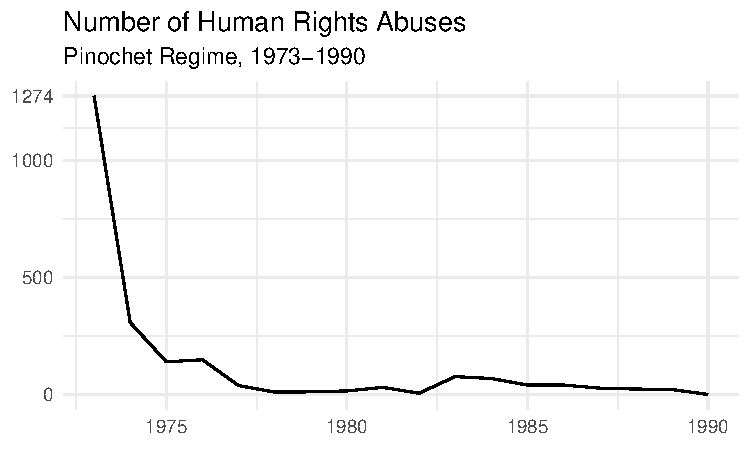
\includegraphics{article_files/figure-latex/time-trend-1} 

}

\caption{Human rights abuses in the Pinochet regime, 1973-1990}\label{fig:time-trend}
\end{figure}

\vspace{.5cm}

We can also explore how the government employed violence across space.
We see that assassinations are concentrated around Santiago and
neighbouring cities. The results are expected. Santiago has been Chile's
most densely populated city since the colonial times and in 1975 the
city was home to about 30\% of the country's population
\citep{un1976yearbook}. Disappearances follow a similar pattern.
Although there are cases in the northern parts of the country, the
military government targeted more victims in Santiago and neighbouring
areas.

\begin{figure}

{\centering 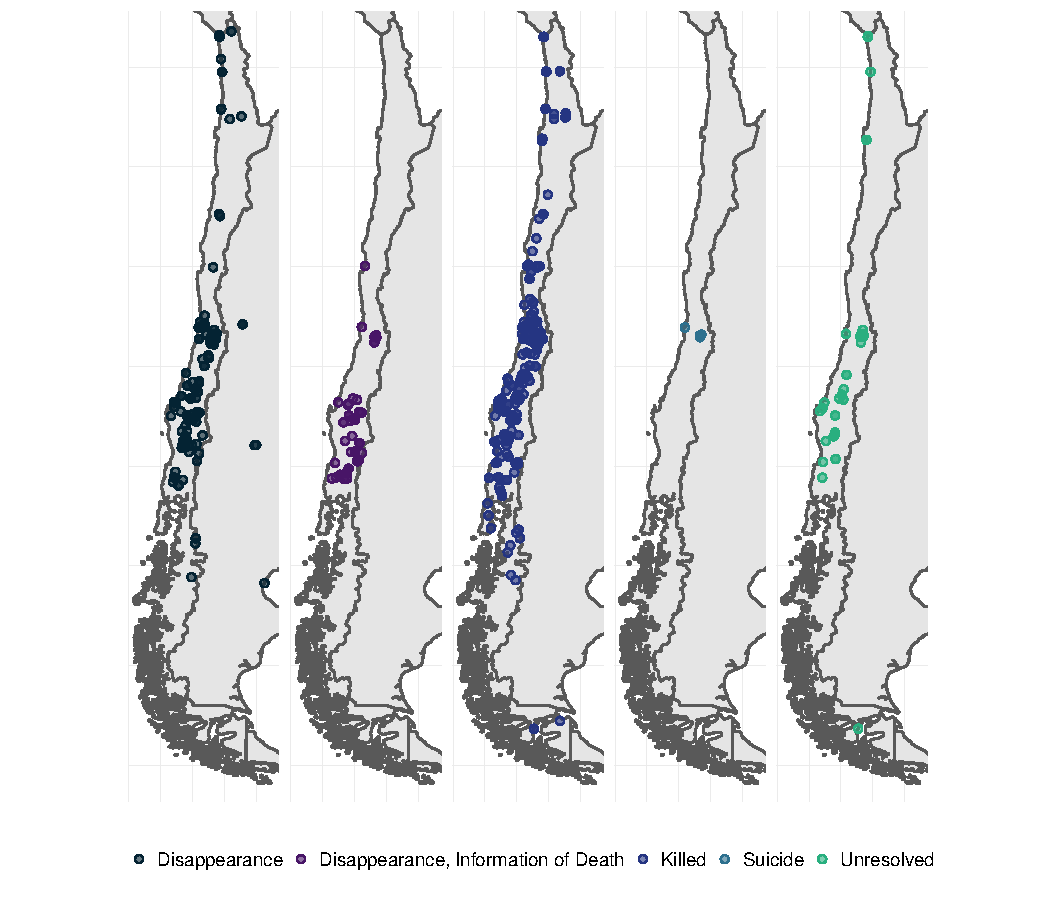
\includegraphics{article_files/figure-latex/maps-1} 

}

\caption{Spatial variation in human rights abuses in the Pinochet regime, 1973-1990}\label{fig:maps}
\end{figure}

We can further disaggregate the analysis and visualise how the regime
persecuted particular groups. School and university students are two
categories of special interest. On 18 September 1073, only one week
after the coup, Pinochet and his followers rounded up thousands of
students and activists in Chile's National Stadium. Military forces
tortured and murdered dozens of prisoners over the course of a few days.
The government again tortured and killed students and activists in its
campaign against the Revolutionary Left Movement (\emph{Movimiento de
Izquierda Revolucionaria}, MIR). The MIR originated in student unions
and in the late 1970s the movement promoted a series of attacks against
government personnel and official buildings. Government forces strongly
retaliated and the group resorted to terrorist tactics to confront the
regime \citep{schlotterbeck2018beyond}.

\vspace{.5cm}

\begin{figure}

{\centering 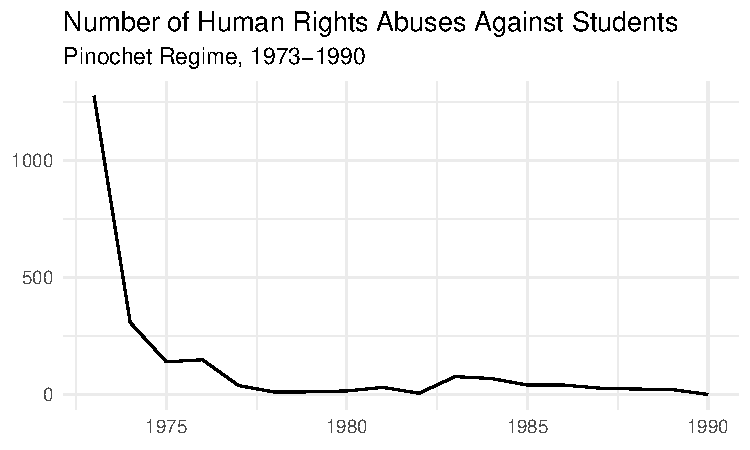
\includegraphics{article_files/figure-latex/time-trend-students-1} 

}

\caption{Human rights abuses against students, 1973-1990}\label{fig:time-trend-students}
\end{figure}

\vspace{.5cm}

\hypertarget{conclusion-new-avenues-for-research}{%
\section{Conclusion: New Avenues for
Research}\label{conclusion-new-avenues-for-research}}

In this paper, we introduce a dataset with rich information about more
than 2,000 victims of the Pinochet regime. Our data come from two
sources. First, we manually coded all information available in the
Report of the Chilean National Commission on Truth and Reconciliation
\citeyearpar{report1991}. Second, we added the geographical locations
and the specific dates of the human rights abuses whenever we could
retrieve them. The graphs and maps included in this article provide some
preliminary results about the temporal and spatial variation of state
violence during Chile's last military government.

We believe our data open new topics of research. For instance,
\citet{lupu2017legacy}, \citet{rozenas2017political} and
\citet{zhukov2018stalin} highlight that state repression has enduring
effects on political preferences and social attitudes. Researchers can
test whether the Pinochet regime has caused similar attitudinal changes
in direct or indirect victims. Moreover, sociologists and criminologists
can analyse the relationship between human rights abuses and post-regime
levels of interpersonal violence. Recent studies show that democracies
which arise after military regimes have higher homicide rates
\citep{frantz2018legacy, karstedt2006democracy}. Our data can show if
areas with significant levels of military repression are more violent
today.

Researchers can also examine how political coalitions affect the use of
lethal violence in authoritarian regimes. Although the topic has
received increasing attention
\citep[e.g.,][]{fjelde2010generals, gandhi2007authoritarian, rivera2017authoritarian},
the internal dynamics of autocratic governments remains understudied.
The main reason is a lack of fine-grained information
\citep[16]{ferrara2014assessing}. By linking human right abuses to
changes in Pinochet's coalition, scholars can explore whether civilian
or bureaucratic support lead to higher incidence of state violence. The
individual data presented here can be combined with government records
at any level of aggregation.

Qualitative scholars will find the personal details of the victims to be
particularly useful. Historians willing to reconstruct the biographies
of specific individuals are able to access pre-compiled information in a
single digital file. Others might be interested in using our data as a
starting point for network analysis or to collect oral testimony from
survivors and acquaintances. In that regard, the dataset can accommodate
future qualitative information. As we include a unique identification
number to each victim, it is easy to update the personal record of any
individual with new data from public archives or personal
correspondence.

Lastly, scholars can investigate the connections between international
legitimacy and domestic politics in repressive regimes. This is a
promising area of research as the Chilean government and American
intelligence services continue to declassify documents from the Pinochet
era. One relevant question is whether pressure from foreign governments
and organisations had any influence over the levels of human rights
abuses in Chile. We hope our dataset is useful for scholars interested
in these and other questions, and that the information it contains
elicits hypotheses not only about the Pinochet period, but about
authoritarian governments more generally.

\newpage
\setlength{\parindent}{0cm}
\setlength{\parskip}{6pt}

\bibliography{references.bib}

\end{document}
